%
%  A few examples
%

\begin {frame} {A few examples}
  \begin {center}
    \includegraphics [height=2cm] {figures/baxter-manipulation.png}
    \hspace*{.7cm}
    \includegraphics [height=2cm] {figures/nextage-demo.png}
  \end {center}
  \begin {center}
    \includegraphics [height=2cm] {figures/fiad-full-run.png}
    \hspace*{.2cm}
    \includegraphics [height=2cm] {figures/romeo-placard.png}
  \end {center}
\end {frame}

%
% Manipulation
%

\begin {frame} {Definitions}

A manipulation motion
\begin {itemize}
\item  is the motion of
  \begin {itemize}
  \item one or several robots and of
  \item one or several objects
  \end {itemize}
\pause
\item such that each object
  \begin{itemize}
  \item either is in a stable position, or
  \item is moved by one or several robots.
  \end {itemize}
\end {itemize}
\end {frame}

\begin {frame} {Composite robot}

Kinematic chain composed of each robot and of each object
\vskip .5cm
\centerline {
  \def\svgwidth {.6\linewidth}
                {\tiny
                  \graphicspath{{./figures/}}
                  \input {figures/composite-robot.pdf_tex}
                }
}
\pause
\vskip .5cm
The configuration space of a composite robot is the cartesian product of the configuration spaces of each robot and object.
$$
\CS = \CS_{r1}\times\cdots\times\CS_{r_{nb\ robots}}\times SE(3)^{nb\ objets}
$$
\end {frame}

%
%  Contraintes numériques
%
\begin {frame} {Numerical constraints}

Constraints to which manipulation motions are subject can be expressed numerically.
\begin{itemize}
\item Numerical constraints:
  $$f (\conf) = 0,\ \ \ \begin{array}{l}m\in\entiernaturel,\\ f\in C^1(\CS,\real^m)\end{array} $$
  \begin{itemize}
    \item \texttt{\scriptsize setConstantRightHandSide(True)}
  \end{itemize}
\item Parameterizable numerical constraints:
  $$f (\conf) = f_0,\ \ \ \begin{array}{l}m\in\entiernaturel,\\ f\in C^1(\CS,\real^m) \\ f_0\in\real^m\end{array} $$
  \begin{itemize}
    \item \texttt{\scriptsize setConstantRightHandSide(False)}
  \end{itemize}
\end{itemize}

\end{frame}

%
%  Exemple
%

\begin {frame} {Example: robot manipulating a ball}
\centerline {
  \parbox {.39\linewidth} {
    \centerline {
      \includegraphics [width=\linewidth] {pictures/ur5-grasp-ball.png}
    }
  }
  \parbox {.05\linewidth} {
    \vskip .5cm
  }
  \parbox {.55\linewidth} {
    \begin{align}
      \CS &= [-\pi,\pi]^6\times \real^3 \\
      \conf &= (q_0,\cdots,q_5,x_{b},y_{b},z_{b})
    \end{align}
    Two \textit{states}:
    \begin{itemize}
    \item \texttt{placement}: the ball is lying on the table,
    \item \texttt{grasp}: the ball is hold by the end-effector.
    \end {itemize}
  }
}
\end {frame}

%
%  Example
%

\begin {frame} {Example: robot manipulating a ball}
\centerline {
  \parbox {.39\linewidth} {
    \centerline {
      \includegraphics [width=\linewidth] {pictures/ur5-grasp-ball.png}
    }
  }
  \parbox {.05\linewidth} {
    \vskip .5cm
  }
  \parbox {.55\linewidth} {
    Each state is defined by a numerical constraint
    \begin{itemize}
    \item \texttt{placement}
      $$
      z_b = 0
      $$
    \pause\item \texttt{grasp}
      $$
      \x_{gripper} (q_0,\cdots,q_5) - \left(\begin{array}{l}x_b\\ y_b\\ z_b\end{array}\right) = 0
        $$
    \end {itemize}
  }
}
Each state is a sub-manifold of the configuration space
\end {frame}

%
%  Example
%

\begin {frame} {Example: robot manipulating a ball}

Motion constraints
\vskip .5cm
\centerline {
  \parbox {.39\linewidth} {
    \centerline {
      \includegraphics [width=\linewidth] {pictures/ur5-grasp-ball.png}
    }
  }
  \parbox {.05\linewidth} {
    \vskip .5cm
  }
  \parbox {.55\linewidth} {
    Two \textit{types of motion}:
    \begin{itemize}
    \item \texttt{transit}: the ball is lying and \textbf{fixed} on the table,
    \item \texttt{transfer}: the ball moves with the end-effector.
    \end {itemize}
  }
}
\end {frame}

%
%  Example
%

\begin {frame} {Example: robot manipulating a ball}

Motion constraints
\vskip .5cm
\centerline {
  \parbox {.39\linewidth} {
    \centerline {
      \includegraphics [width=\linewidth] {pictures/ur5-grasp-ball.png}
    }
  }
  \parbox {.05\linewidth} {
    \vskip .5cm
  }
  \parbox {.55\linewidth} {
    \begin{itemize}
    \item \texttt{transit}
      $$
      \begin{array}{lcl}
      \begin{array}{lcl}
        x_b &=& x_0 \\
        y_b &=& y_0 \\
      \end{array}& \left.\right\}&\mbox {parameterizable} \\
      \begin{array}{lcl}
        z_b = 0
      \end{array}&\left.\right\}& \mbox {simple}
      \end {array}
        $$
    \item \texttt{transfer}
      $$
      \x_{gripper} (q_0,\cdots,q_5) - \left(\begin{array}{l}x_b\\ y_b\\ z_b\end{array}\right) = 0
        $$
    \end {itemize}
  }
}
\end {frame}

%
%  Feuilletage
%

\begin {frame} {Foliation}
  Motion constraints define a foliation of the admissible configuration space (\texttt{grasp} $\cup$ \texttt{placement}).
  \begin{columns}
    \centering
    \column{0.5\textwidth}
    \def\svgwidth {\linewidth}
                  {\tiny
                    \graphicspath{{./figures/}}
                    \input {figures/foliation-example.pdf_tex}
                }
    \column{0.5\textwidth}
    \centering
    \begin{itemize}
    \item $f$: position of the ball
      $$L_{f}(f_1) = \left\{\conf\in\CS, f (\conf) = f_1 \right\}$$
    \item $g$: grasp of the ball
      $$L_{g}(0) = \left\{\conf\in\CS, g (\conf) = 0 \right\}$$
    \end{itemize}
  \end {columns}

\end {frame}

%
%  Feuilletage
%

\begin {frame} {Foliation}
  Motion constraints define a foliation of the admissible configuration space (\texttt{grasp} $\cup$ \texttt{placement}).
  \begin{columns}
    \centering
    \column{0.5\textwidth}
    \def\svgwidth {\linewidth}
                  {\tiny
                    \graphicspath{{./figures/}}
                    \input {figures/foliation-path.pdf_tex}
                }
    \column{0.5\textwidth}
    \centering
    Solution to a manipulation planning problem is a concatenation of \textit{transit} and \textit{transfer} paths.
  \end {columns}

\end {frame}

%
%  General case
%

\begin {frame} {General case}

  In a manipulation problem,
  \begin{itemize}
  \item the state of the system is subject to
    \begin {itemize}
      \item numerical constraints
    \end {itemize}
    \pause
  \item trajectories of the system are subject to
    \begin {itemize}
    \item numerical constraints
    \item parameterizable numerical constraints.
    \end {itemize}
  \end{itemize}
\end {frame}

%
%  General case
%

\begin {frame} {General case}

  \vskip .55cm
  In a manipulation problem,
  \begin{itemize}
  \item the state of the system is subject to
    \begin {itemize}
      \item numerical constraints
    \end {itemize}
  \item trajectories of the system are subject to
    \begin {itemize}
    \item \sout{numerical constraints}
    \item parameterizable numerical constraints, the dimension of the parameter being possibly less than the dimension of the constraint.
    \pause\item parameter value is constant along trajectories.
    \end {itemize}
  \end{itemize}
\end {frame}

%
%  Constraint graph
%

\begin {frame} {Constraint graph}
  A manipulation planning problem can be represented by a \textit{manipulation graph}.
  \begin {itemize}
    \item \textbf{Nodes} or \textit{states} are numerical constraints.
    \item \textbf{Edges} or \textit{transitions} are parameterizable numerical constraints.
  \end {itemize}
  \begin{center}
      \begin{tikzpicture}[>=stealth',auto,node distance=3.5cm,
        thick,main node/.style={circle,draw,text width=1.5cm,align=center,font=\footnotesize}]
        {\node[main node] (nh) {Placement};}
        {\node[main node] (h) [right of=nh] {Grasp};}
        {\path[->] (nh) edge[loop left] node[left, align=right] {Transit} (nh);}
        {\path[<-] (h) edge[bend right=45] node[above] {Grasp ball} (nh);}
        {\path[->] (h) edge[bend left=45] node[below] {Release ball} (nh);}
        {\path[->] (h) edge[loop right] node[right] {Transfer} (h);}
      \end{tikzpicture}
    \end{center}
\end {frame}

%
%  Projecting configuration on constraint
%

\begin {frame} {Projecting configuration on constraint}
  Newton-Raphson algorithm
  \begin {itemize}
  \item $\conf_0$ configuration,
  \item $f(\conf) = 0$ non-linear constraint,
  \item $\epsilon$ numerical tolerance
  \end {itemize}
  Projection ($\conf_0, f$):
  \begin{itemize}
    \item [] $\conf = \conf_0$; $\alpha = 0.95$
    \item [] for i from 1 to max\_iter:
      \begin {itemize}
      \item [] $\conf = \conf - \alpha \left(\frac {\partial f}{\partial \conf}(\conf)\right)^{+} f (\conf)$
      \item [] if $\|f(\conf)\| < \epsilon$: return $\conf$
      \end {itemize}
    \item [] return failure
  \end{itemize}

\end {frame}

%
%  Steering method
%

\begin {frame} {Steering method}
  Mapping $\steer$ from $\CS\times\CS$ to $C^1([0,1],\CS)$ such that
  \begin {align*}
    \steer (\conf_0,\conf_1) (0) &= \conf_0 \\
    \steer (\conf_0,\conf_1) (1) &= \conf_1 \\
  \end {align*}
\end {frame}

%
%  Constrained steering method
%

\begin {frame} {Constrained steering method}
  Let
  \begin {itemize}
  \item $\steer$ be a steering method
  \item $f\in C^1(\CS,\real^m)$ be a numerical constraint.
  \end {itemize}
  A constrained steering method $\bar{\steer}$ of constraint $f$ is a steering method such that
  \begin {align*}
    \forall t\in [0,1], f(\bar{\steer} (t)) &= 0
  \end {align*}
  \pause
  It can be defined by projection
  $$\bar{\steer} = proj\circ \steer
  $$
\end {frame}

\begin {frame} {Projecting path on constraint}
  \begin {itemize}
  \item $path$: mapping from $[0,1]$ to $\CS$
  \item $f(\conf) = 0$ non-linear constraint,
  \end {itemize}
  Applying Newton Raphson at each point may result in a discontinuous path
  \begin {center}
  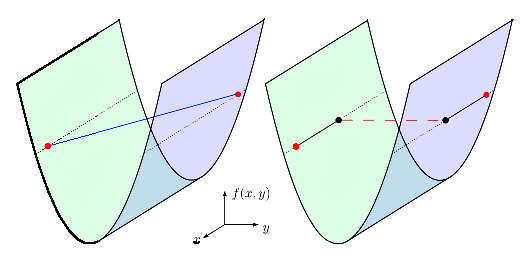
\includegraphics [width=.5\linewidth]{figures/second_order_polynomial2.eps}
  \end {center}
\end {frame}

%
%  Discontinuous Projection
%

\begin {frame} {Discontinuous Projection}
  \begin {center}
  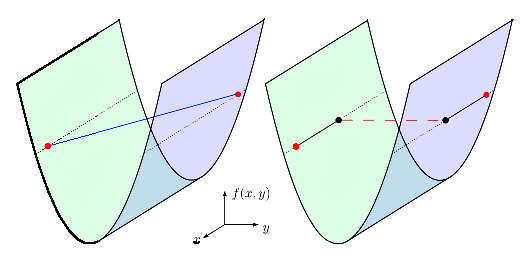
\includegraphics [width=.5\linewidth]{figures/second_order_polynomial2.eps}
  \end {center}
  \begin{align*}
  \CS=\real^2,\, & f(x,y) = y^2-1\\
  &\frac{\partial f}{\partial \conf} = \left(\begin{array}{ll}
  0 & 2y\end{array}\right),\ 
  \frac{\partial f}{\partial \conf}^{+} = \left(\begin{array}{l}
  0 \\ \frac{1}{2y}\end{array}\right)\ \mbox{ou} \left(\begin{array}{l}
  0 \\ 0\end{array}\right)\\
  & y_{i+1} = y_i + \frac {1-y_i^2}{2y_i}
  \end{align*}
\end {frame}

%
%  Testing projection continuity
%

\begin {frame} {Testing projection continuity}
  \begin{columns}
    \centering
    \column{0.7\textwidth}
    \begin {itemize}
      \item The initial path is sampled and successive samples are projected,
      \item {\color {white} if 2 successive projections are too far away, an intermediate sample is selected.}
      \item {\color {white} Choosing appropriate sampling ensures us continuity of the projection.}
    \end {itemize}
    \column{0.3\textwidth}
    \begin {center}
      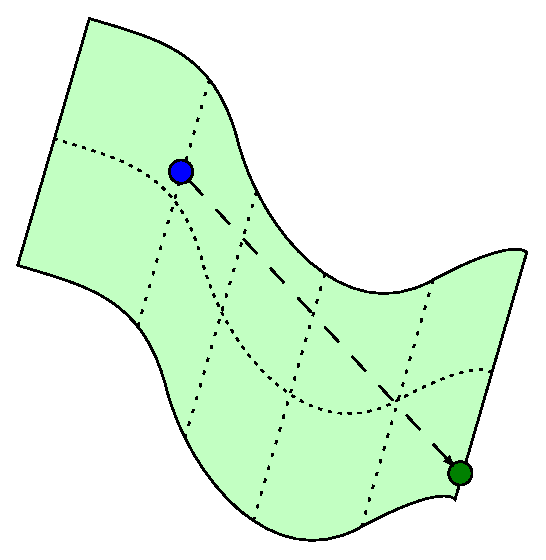
\includegraphics [width=.9\linewidth] {figures/progressive_0.eps}
    \end {center}
  \end {columns}
\end {frame}

%
%  Testing projection continuity
%

\begin {frame} {Testing projection continuity}
  \begin{columns}
    \centering
    \column{0.7\textwidth}
    \begin {itemize}
      \item The initial path is sampled and successive samples are projected,
      \item {\color {white} if 2 successive projections are too far away, an intermediate sample is selected.}
      \item {\color {white} Choosing appropriate sampling ensures us continuity of the projection.}
    \end {itemize}
    \column{0.3\textwidth}
    \begin {center}
      \includegraphics [width=.9\linewidth] {figures/progressive_1.eps}
    \end {center}
  \end {columns}
\end {frame}

%
%  Testing projection continuity
%

\begin {frame} {Testing projection continuity}
  \begin{columns}
    \centering
    \column{0.7\textwidth}
    \begin {itemize}
      \item The initial path is sampled and successive samples are projected,
      \item {\color {white} if 2 successive projections are too far away, an intermediate sample is selected.}
      \item {\color {white} Choosing appropriate sampling ensures us continuity of the projection.}
    \end {itemize}
    \column{0.3\textwidth}
    \begin {center}
      \includegraphics [width=.9\linewidth] {figures/progressive_2.eps}
    \end {center}
  \end {columns}
\end {frame}

%
%  Testing projection continuity
%

\begin {frame} {Testing projection continuity}
  \begin{columns}
    \centering
    \column{0.7\textwidth}
    \begin {itemize}
      \item The initial path is sampled and successive samples are projected,
      \item {if 2 successive projections are too far away, an intermediate sample is selected.}
      \item {\color {white} Choosing appropriate sampling ensures us continuity of the projection.}
    \end {itemize}
    \column{0.3\textwidth}
    \begin {center}
      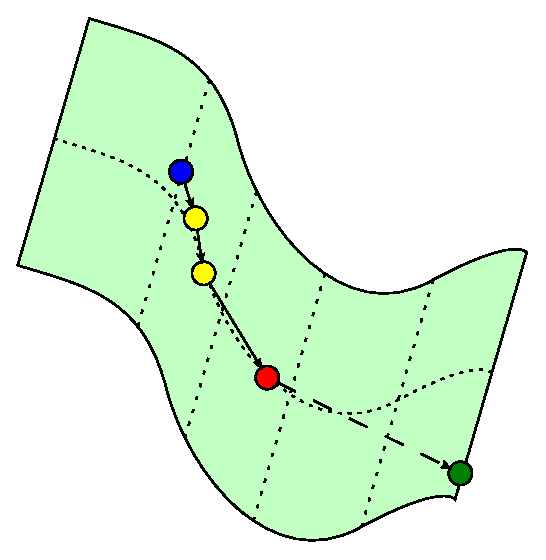
\includegraphics [width=.9\linewidth] {figures/progressive_3.eps}
    \end {center}
  \end {columns}
\end {frame}

%
%  Testing projection continuity
%

\begin {frame} {Testing projection continuity}
  \begin{columns}
    \centering
    \column{0.7\textwidth}
    \begin {itemize}
      \item The initial path is sampled and successive samples are projected,
      \item {if 2 successive projections are too far away, an intermediate sample is selected.}
      \item {Choosing appropriate sampling ensures us continuity of the projection.}
    \end {itemize}
    \column{0.3\textwidth}
    \begin {center}
      \includegraphics [width=.9\linewidth] {figures/progressive_4.eps}
    \end {center}
  \end {columns}
\end {frame}

%
%  Exploration de l'espaces des configurations admissibles
%

\begin{frame}[fragile]{Algorithm}{Manipulation RRT}
%-------------------------------------------------------
  \begin{columns}
    \column{0.3\textwidth}
    \includegraphics<1>[width=\textwidth,height=\textheight,keepaspectratio]{img/mrrt/foliation-project-seq-1.png}
    \includegraphics<2-3>[width=\textwidth,height=\textheight,keepaspectratio]{img/mrrt/foliation-project-seq-2.png}
    \includegraphics<4>[width=\textwidth,height=\textheight,keepaspectratio]{img/mrrt/foliation-project-seq-3.png}
    \includegraphics<5>[width=\textwidth,height=\textheight,keepaspectratio]{img/mrrt/foliation-project-seq-4.png}
    \includegraphics<6>[width=\textwidth,height=\textheight,keepaspectratio]{img/mrrt/foliation-project-seq-5.png}
    \includegraphics<7->[width=\textwidth,height=\textheight,keepaspectratio]{img/mrrt/foliation-project-seq-5.png}
    \column{0.7\textwidth}
    \begin{block}{Manipulation RRT}
      \setbeamertemplate{itemize item}{}% Remove bullets frp, ote,oze sinote,
      \setlength\leftmargini{0em}
      \begin{itemize}[leftmargin=*]
        \item<1-> $\conf_{rand}$ = shoot\_random\_config()
        \item <2-> for each connected component:
          \setlength\leftmargin{0em}
          \begin{itemize}[leftmargin=*]
          \item[]<2-> $\conf_{near}$ = nearest\_neighbor($\conf_{rand}$, $roadmap$)
          \item[]<3-> $T$ = select\_transition($\conf_{near}$)
          \item[]<4-> $\conf_{proj}$ = generate\_target\_config($\conf_{near},\conf_{rand}$, $T$)
          \item[]<5-> $\conf_{new}$ = extend($\conf_{near}$, $\conf_{proj}$, $T$)
          \item[]<6-> $roadmap$.insert\_node($\conf_{new}$)
          \item[]<7-> $roadmap$.insert\_edge($T$, $\conf_{near}$, $\conf_{new}$)
          \item[]<7-> new\_nodes.append ($\conf_{new}$)
          \end{itemize}
        \item <8-> for $\conf\in (\conf_{new}^1, ..., \conf_{new}^{n_{cc}})$:
          \begin{itemize}
            \item[]<9-> connect ($\conf$, roadmap)
          \end{itemize}
      \end{itemize}
    \end{block}
  \end{columns}
\end{frame}

%
%  Select transition
%

\begin {frame} {Select transition}

  $T$ = select\_transition($\conf_{near}$)
  \vskip .5cm

  Outward transitions of each state are given a probability distribution. The transition from a state to another state is chosen by random sampling.
  \begin{center}
      \begin{tikzpicture}[>=stealth',auto,node distance=3.5cm,
        thick,main node/.style={circle,draw,text width=1.5cm,align=center,font=\footnotesize}]
        {\node[main node] (nh) {Placement};}
        {\node[main node] (h) [right of=nh] {Grasp};}
        {\path[->] (nh) edge[loop left] node[left, align=right] {Transit} (nh);}
        {\path[<-] (h) edge[bend right=45] node[above] {Grasp ball} (nh);}
        {\path[->] (h) edge[bend left=45] node[below] {Release ball} (nh);}
        {\path[->] (h) edge[loop right] node[right] {Transfer} (h);}
      \end{tikzpicture}
    \end{center}
\end {frame}

%
%  Generate target configuration
%

\begin {frame} {Generate target configuration}

$\conf_{proj}$ = generate\_target\_config($\conf_{near},\conf_{rand}$, $T$)
\vskip .5cm
Once transition $T$ has been selected, $\conf_{rand}$ is \textit {projected} onto the destination state $S_{dest}$ in a configuration reachable by $\conf_{near}$.
\begin{align*}
  f_{T} (\conf_{proj}) &= f_{T} (\conf_{near})\\
  f_{S_{dest}} (\conf_{proj}) &= 0
\end{align*}
\end {frame}

%
%  Extend
%

\begin {frame} {Extend}

$\conf_{new}$ = extend($\conf_{near}$, $\conf_{proj}$, $T$)
\vskip.5cm
\textit {Project} straight path $[\conf_{near},\conf_{proj}]$ on transition constraint:
\begin {itemize}
\item if projection successful and projected path collision free
$$
\conf_{new} \leftarrow \conf_{proj}
$$
\pause
\item otherwise $(\conf_{near},\conf_{new})\leftarrow$ largest path interval tested as collision-free with successful projection.
\end {itemize}
\pause
$$
\forall \conf\in(\conf_{near},\conf_{new}),\ f_{T} (\conf) = f_{T}(\conf_{near})
$$
\end {frame}

%
%  Connect
%

\begin {frame} {Connect}

  \begin{block}{connect ($\conf$, roadmap)}
    \setbeamertemplate{itemize item}{}% Remove bullets frp, ote,oze sinote,
    \begin{itemize}
    \item <1-> for each connected component $cc$ not containing $\conf$:
        \begin{itemize}
        \item []<1->for all $n$ closest config $\conf_1$ to $\conf$ in $cc$:
          \begin{itemize}
          \item connect ($\conf$, $\conf_1$)
          \end{itemize}
        \end{itemize}
    \end{itemize}
  \end{block}
\end {frame}

%
%  Connect
%

\begin {frame} {Connect}
connect ($\conf_0$, $\conf_1$):
\begin{itemize}
  \item [] $S_0$ = state ($\conf_0$)
  \item [] $S_1$ = state ($\conf_1$)
  \item [] $T$ = transition ($S_0$, $S_1$)
  \item [] if $T$ and $f_{T} (\conf_0) == f_{T} (\conf_1)$:
    \begin {itemize}
    \item [] if p = projected\_path ($T$, $\conf_0$, $\conf_1$) collision-free:
      \begin {itemize}
        \item [] roadmap.insert\_edge ($T$, $\conf_0$,$\conf_1$)
      \end {itemize}
    \end {itemize}
  \item [] return
\end{itemize}

\end {frame}

%
%  Connecting trees
%

\begin {frame} {Connecting trees}
Manipulation RRT is initialized with $\conf_{init}$, $\conf_{goal}$.
\begin {itemize}
\item 2 connected components.
\item possible connection.
\end {itemize}
\centerline {
  \def\svgwidth {\linewidth}
                {
                  \graphicspath{{./figures/}}
                  \input {figures/connecting-trees-simple-grasp.pdf_tex}
                }
}
\end{frame}

%
%  Connecting trees general case
%

\begin {frame} {Connecting trees: general case}
Manipulation RRT is initialized with $\conf_{init}$, $\conf_{goal}$.
\begin {itemize}
\item 2 connected components,
\item no possible connection.
\end {itemize}
\centerline {
  \def\svgwidth {\linewidth}
                {
                  \graphicspath{{./figures/}}
                  \input {figures/connecting-trees.pdf_tex}
                }
}
\end{frame}

%
%  Connecting trees general case
%

\begin {frame} {Connecting trees: general case}
Manipulation RRT is initialized with $\conf_{init}$, $\conf_{goal}$.
\begin {itemize}
\item 2 connected components,
\item no possible connection.
\end {itemize}
\begin {columns}
\column {.5\textwidth}
\centerline {
  \def\svgwidth {\linewidth}
                {\tiny
                  \graphicspath{{./figures/}}
                  \input {figures/connecting-trees.pdf_tex}
                }
}
\column {.5\textwidth}
  \begin{center}
    \tiny
      \begin{tikzpicture}[>=stealth',auto,node distance=1.75cm,
        thick,main node/.style={circle,draw,text width=.75cm,align=center,
          font=\tiny}]
        {\color{red}\node[main node] (nh) {Placement};}
        {\color{blue}\node[main node] (h) [right of=nh] {Grasp};}
        {\color{red}\path[->] (nh) edge[loop left] node[left, align=right] {Transit} (nh);}
        {\color{red}\path[<-] (h) edge[bend right=22.5] node[above] {Grasp ball} (nh);}
        {\color{blue}\path[->] (h) edge[bend left=22.5] node[below] {Release ball} (nh);}
        {\color{blue}\path[->] (h) edge[loop right] node[right] {Transfer} (h);}
      \end{tikzpicture}
    \end{center}
\end {columns}
\end{frame}

%
%  Generate target configuration
%

\begin {frame} {Crossed foliation transition: generate target configuration}

  \begin {columns}
    \column {.6\linewidth}
    $\conf_{proj}$ = generate\_target\_config($\conf_{near},\conf_{rand}$, $T$)
    \vskip .5cm
    $\conf_1\leftarrow$ pick configuration
    \begin {itemize}
    \item in state $S_1$,
    \item not in same connected component as $\conf_{near}$
    \end {itemize}
    \begin{align*}
      f_{T_1} (\conf_{proj}) &= f_{T_1} (\conf_{near})\\
      {\color{red} f_{T_2} (\conf_{proj})} &{\color{red}= f_{T_2} (\conf_1)}\\
      f_{S_2} (\conf_{proj}) &= 0
    \end{align*}
    \column {.4\linewidth}
    \begin{center}
      \tiny
      \begin{tikzpicture}[>=stealth',auto,node distance=3.25cm,
          thick,main node/.style={circle,draw,text width=1.25cm,align=center,
            font=\tiny}]
        {\node[main node] (nh) {$S_1$};}
        {\node[main node] (h) [right of=nh] {$S_2$};}
        {\path[<-] (h) edge[bend right=0] node[above] {Crossed foliation}
          (nh);}
        {\path[<-] (h) edge[bend right=22.5] node[above] {$T_1$} (nh);}
        {\path[->] (h) edge[bend left=22.5] node[below] {$T_2$} (nh);}
      \end{tikzpicture}
    \end{center}
  \end {columns}
\end {frame}

%
%  Extend
%

\begin {frame} {Crossed foliation transition: extend}

  $\conf_{new}$ = extend($\conf_{near}$, $\conf_{proj}$, $T_1$)
  \vskip.5cm
  \textit {Project} straight path $[\conf_{near},\conf_{proj}]$ on $T_1$ constraint:
  \begin {itemize}
  \item if projection successful and projected path collision free
    $$
    \conf_{2} \leftarrow \conf_{proj}
    $$
    \pause
    \begin{align*}
      f_{T_2} (\conf_{2}) &= f_{T_2} (\conf_1)\\
      f_{S_2} (\conf_{2}) &= 0
    \end{align*}
    \item $\conf_2$ is connectable to $\conf_1$ via $T_2$.
    \end{itemize}
\end {frame}

%
%  Relative positions as numerical constraints
%

\begin {frame} {Relative positions as numerical constraints}

  \centerline{
    \parbox{.5\linewidth}{
      \begin{itemize}
      \item $T_1 = T_{(R_1,t_1)}\in SE(3)$, $T_2 = T_{(R_2,t_2)}\in SE(3)$.
      \item $T_{2/1} = T_1^{-1}\circ T_2$ can be represented by a vector of dimension 6:
      $$
      \left(\begin{array}{c} \mathbf{u} \\ \mathbf {v}\end{array}\right)
      $$
      where
      $$
      \mathbf{u} = R_1^T (t_2-t_1)
      $$
      $R_1^T R_2$  matrix of the rotation around axis $\mathbf{v}/\|\mathbf {v}\|$ and of angles $\|\mathbf {v}\|$.
      \end{itemize}
    }
    \parbox{.5\linewidth}{
      \centerline {
        \def\svgwidth {\linewidth}
                      {\tiny
                        \graphicspath{{./figures/}}
                        \input {figures/relative-pose.pdf_tex}
                      }
      }
    }
  }
\end {frame}

